In recent years, cryptocurrencies such as Bitcoin, Ether, and Dogecoin have gained increasing attention in the financial world. In particular, the first cryptocurrency called Bitcoin - developed by an unknown individual or group under the pseudonym Satoshi Nakamoto and first presented in 2009 \cite{Bitcoin2009} - has achieved a market cap of about $750$ billion United States dollar (USD) as of \date{14 June 2021}. This is comparable to the market cap at the stock market of companies like Facebook and Tesla \cite{MarketCapCompany2021}\cite{MarketCapBitcoin2021}.\\

Bitcoin is mostly used as a form of digital money. Each Bitcoin transaction between two parties is stored on the Bitcoin blockchain. A simplified illustration of the Bitcoin blockchain is depicted in Fig.~\ref{fig:blockchain}. The Bitcoin blockchain is an ordered chain of blocks, where each block contains data on Bitcoin transactions. New blocks are created by investing computing power in solving a mathematical task. The person or group that solves the task first is rewarded with new Bitcoins as well as with the transaction fees of the transactions in the new block. The new block is appended to the Bitcoin blockchain. This whole process is called Bitcoin mining because it implies the creation of new Bitcoins.

\begin{figure}[h]
  \centering
  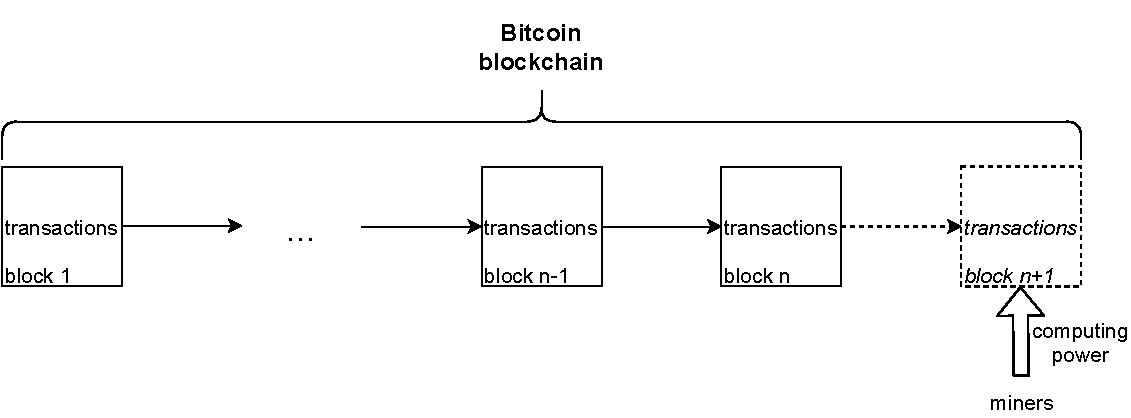
\includegraphics[width=\textwidth]{bitcoin_blockchain.pdf}
  \caption{Simplified illustration of the Bitcoin blockchain. The blocks contain all transactions made with the cryptocurrency Bitcoin. A new block $n+1$ is created by investing computing power to solve a mathematical task. The person or group that solves this task first is rewarded with new Bitcoins as well as with the transactions fees of the transactions in the new block. The new block $n+1$ is appended to the Bitcoin blockchain. This process is called Bitcoin mining as it implies the creation of new Bitcoins.}
  \label{fig:blockchain}
\end{figure}

Besides its original purpose as a form of digital money, Bitcoins are treated as a financial asset that is exchanged with other currencies, e.g. USD, at cryptocurrency exchanges such as Binance, Kraken, and Coinbase. The market price of Bitcoin - e.g. expressed in USD - is a result of demand and supply as the creation of Bitcoins requires computing power as its underlying value. \\

For traders, it is of interest to be able to predict the future development of the Bitcoin market price in order to maximize returns.
The present work is concerned with the prediction of the direction of the Bitcoin market price one day into the future based on information from the current and past days. The direction is either \enquote{up} if the Bitcoin market price is expected to increase, or \enquote{down} if it is expected to decrease. Thus, here, the prediction of the Bitcoin market price is treated as a binary classification problem.\\

In Section~\ref{sec:dataset}, a time series dataset of the Bitcoin market price and related measures is developed. A transformation of this dataset to the above described classification task allows an application of supervised machine learning techniques. In the present paper, a simple majority predictor, a logistic regression, the K-nearest neighbors algorithm, as well as a deep neural network are applied. A brief description of these techniques is given in Section~\ref{sec:theory}. In addition, the split of the dataset into training, validation, and test examples as well as cross-validation as evaluation techniques are presented. In Section~\ref{sec:implementation_software}, a list of the applied software is given, and particularities of the implementation are described. The classification results are described in Section~\ref{sec:results}. A comparison of the different classification techniques is given in Section~\ref{sec:discussion}. Finally, in Section~\ref{sec:conclusion_outlook}, the results of the present work are summarized and an outlook on further objects of research is given.